The inflation gas is key to providing the structural stiffness for the inflatable: it is required to bring all members into tension to prevent skin wrinkling under compressive loading. To this end, the aeroshell will require an inflation system that is reliable, lightweight and fitting within mass and volume constraints. This subsection details the selection of an inflation gas and design of the inflation system upon which aeroshell deceleration capability hinges.

\subsubsection{Gas generator selection}
Inflation systems can be categorized as tanked-gas systems, phase-change systems and chemical gas-generation systems \cite{Jenkins2001}. These systems have each been considered for their respective advantages, yielding a tanked nitrogen inflation system as outcome. 

%\paragraph{Phase-change system}
Phase-change systems have the potential to provide significant weight reductions. The most promising option is a liquid hydrogen inflation system, while other phase-change systems involve subliming powders, although these are incapable of achieving high pressures \cite{Freeland1998}.  On the basis of system mass fractions investigated by Brown et al. \cite{Brown2009} and the mass estimation tool detailed in section \ref{subsec:structool}, a structural mass reduction of nearly 20 [$kg$] is deemed feasible with a cryogenic liquid hydrogen inflation system following from the mass estimation tool formulated in section \ref{subsec:structool}. 

This mass reduction comes at the expense of reliability, however. These systems involve a phase-change process, inherently unpredictable and thereby accompanied with reduced inflation system reliability \cite{Jenkins2001}. In addition, cryogenic storage requires profound thermal control to keep it below its required temperature. While this poses a challenge for orbiting satellites, it is even more so an issue in the heated re-entry environment of the inflatable aeroshell. Reliability is further lessened by the absence of successful efforts in the past to accommodate a phase-change inflation system in spaceflight, let alone a high-pressure application like the aeroshell at hand. As reliability is key for transporting human payload, phase-change systems are deemed ill-suited. Moreover, a liquid hydrogen inflation system poses issues for safety when operating in the Earth atmosphere, in which flammability risk is present by the dual presence of hydrogen and oxygen in a heated environment.

%\paragraph{Chemical gas-generation system
Chemical gas-generation systems similarly feature a higher level of complexity and thereby lower level of reliability than tanked-gas systems \cite{Jenkins2001}. Moreover, while weight reductions are deemed feasible, these involve the use of hydrazine \cite{Jenkins2001, Freeland1998}. Hydrazine poses issues with respect to cost and handling, but most importantly with respect to sustainability. As the decelerator will make contact with a hard surface, leakage of hydrazine into the Martian atmosphere and pollution of the landing site by its toxic nature poses a risk. This risk would violate \gls{cospar} regulations and moreover limit the sustainable dimension of the mission.

Tanked-gas systems are the preferred choice, featuring a significantly higher level of reliability and past application. Most notably, these have seen application in the \gls{irve} missions in the form of a nitrogen blow-down system \cite{Smith2010}. Blow-down systems offer controllable gas flow at low development and hardware cost \cite{Freeland1998}. Moreover, these are excellently suited for high-pressure applications in inflatable structures \cite{Jenkins2001}.



\subsubsection{Gas generator design and sizing}
A nitrogen tank is used for storage and supply of nitrogen gas. The minimum inflation pressure in the toroids is based on the premise that it should counteract the aerodynamic force exerted to bring flexible material into tension, formulated in Equation \ref{eq:Pmin}. The volume that is inflated may be approximated and follows from Equation \ref{eq:volume}.

\begin{equation}
V = \sum_{i=1}^{7} wh ???
\label{eq:volume}
\end{equation}

It follows that a pressure of  ??? [$Pa$] over a total volume of ??? [$m^{3}$] is required in the inflatable bladders. Based on the thermal analysis presented in subsection \ref{subsec:infldes}, the gas will be exposed to a temperature of approximately ??? [$K$] during operation. Via the ideal gas law, the total mass is then calculated as ??? [$kg$] given a molar mass of 22 [$g/mole$] for nitrogen gas \cite{Samareh2011}.

This yields the total gas that is to be held within the pressure tank. An additional contingency of 25 $\%$ is taken into account for leakage, which requires additional gas flow to make up for the lost volume, so called make up gas \cite{Jenkins2001}.

\subsubsection{Inflation system integration}


Figure \ref{fig:infsys} shows a schematic representation of the inflation system. Moving from left to right the inflation gas is stored in a the nitrogen tank. Pressure and temperature sensors are included to monitor the storage conditions. A separate valve is included for filling purposes of the tank, and a release valve is included for emptying the tank outside normal mission operations. A electromechanical valve release the pressure. A electromechanical valve is used since it allows for multiple uses as opposed to for example pyrotechnical valves. From the high pressure within the storage tank the controlled the pressure is reduced and more precisely controlled by a set of two pressure regulators (including internal release valves). A set of check valves, allowing flow only in one direction, connects to the toroid. The toroids are grouped together and not connected all at once. This allows for partial function if a leakage occurs in of the groups. The check valves prevent the flow from equilibrating over the toroids in this case.

A final set of check valves is included to connect the toroids to the vent. This allows for reducing the pressure in case it becomes to high. The conditions within the tank are measured by a set of pressure and temperature transducers. If the pressure becomes to high, for example due to the thermal heating the vent functions to lower the pressure. Pressure transducer however are also important for making sure the minimum pressure is maintained since the pressure can drop due to leakage. 

\begin{figure}[h]
		\centering
		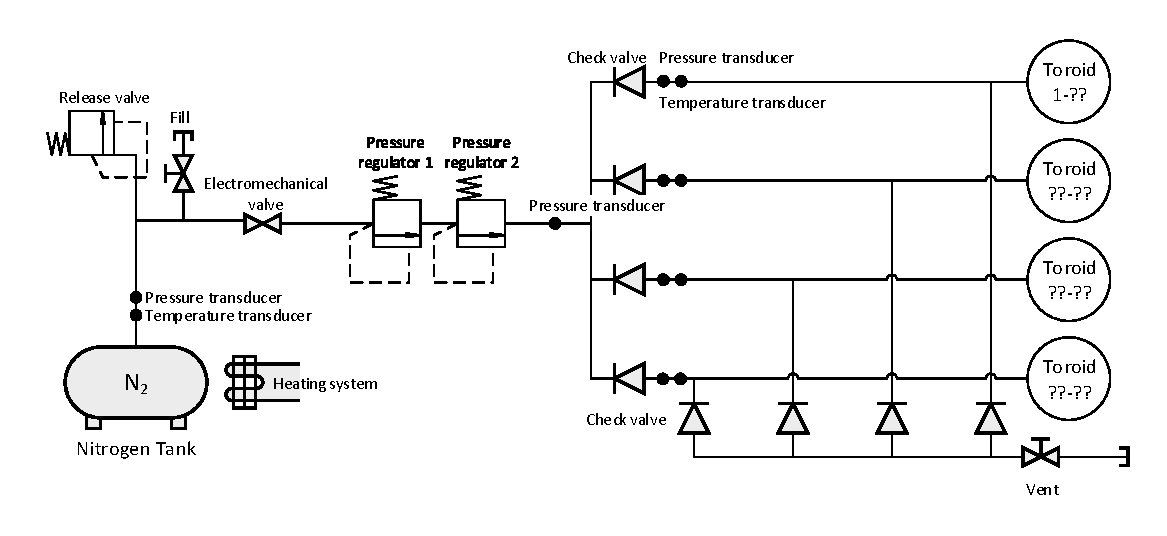
\includegraphics[width=1.0\textwidth]{./Figure/Structure/infsys.pdf}
		\caption{Schematic view of the inflation system (adapted from \cite{Hughes2005})}
		\label{fig:infsys}
\end{figure}






